\documentclass[a4paper,12pt]{article}
\usepackage[utf8]{inputenc}
\usepackage[spanish]{babel}
\usepackage{color}
\usepackage{parskip}
\usepackage{graphicx}
\usepackage{multirow}
\usepackage{listings}
\usepackage{vmargin}
\usepackage{datetime}
\newdate{date}{2}{11}{2017}
\graphicspath{ {imagenes/} }
\definecolor{mygreen}{rgb}{0,0.6,0}
\definecolor{lbcolor}{rgb}{0.9,0.9,0.9}
\usepackage{epstopdf}
\usepackage{float}


\setpapersize{A4}
\setmargins{2.5cm}       % margen izquierdo
{1.5cm}                        % margen superior
{16.5cm}                      % anchura del texto
{23.42cm}                    % altura del texto
{10pt}                           % altura de los encabezados
{1cm}                           % espacio entre el texto y los encabezados
{0pt}                             % altura del pie de página
{2cm}     

\lstset{
    tabsize=4,    
%   rulecolor=,
    language=[GNU]C++,
        basicstyle=\tiny,
        aboveskip={1.5\baselineskip},
        columns=fixed,
        showstringspaces=false,
        extendedchars=false,
        breaklines=true,
        prebreak = \raisebox{0ex}[0ex][0ex]{\ensuremath{\hookleftarrow}},
        frame=single,
        showtabs=false,
        showspaces=false,
        showstringspaces=false,
        identifierstyle=\ttfamily,
        keywordstyle=\color[rgb]{0,0,1},
        commentstyle=\color[rgb]{0.026,0.112,0.095},
        stringstyle=\color{red},
        numberstyle=\color[rgb]{0.205, 0.142, 0.73},
%        \lstdefinestyle{C++}{language=C++,style=numbers}’.
}


\begin{document}
\title{Scanner de Tokens}
\author{
Christofer Fabián Chávez Carazas \\
\small{Universidad Nacional de San Agustín de Arequipa} \\
\small{Escuela Profesional de Ciencia de la Computación} \\
\small{Compiladores}
}
\date{\displaydate{date}}

\maketitle

\begin{large}
 \textbf{Problema}
\end{large}

\textbf{Desarrollar un scanner que reconozca lo siguiente:}

\begin{itemize}
 \item ID
 \item NUM
 \item $+,\:-,\:*,\:/$
 \item $>,\:>=,\:<,\:>=,\:=,\:==,\:!=$
 \item $\{,\:\},\:[,\:],\:",\:;,\:(,\:)$
 \item Ignorar Comentario de línea y de bloque.
\end{itemize}

\begin{large}
 \textbf{Programa}
\end{large}

\begin{itemize}
 \item \textbf{scanner.h}

 Primero se verifica que el flag \textit{comentario} está activado, para seguir con el scanner o descartar el caracter. Si está activado se verifica si se desactiva con un
 salto de línea (comentario de línea) o con un ``*/'' (comentario de bloque). Si es que el flag está desactivado se procede a verificar el caracter. Primero se verifica si es
 un dígito, si sí lo es entonces se proceso más caracteres hasta dejar de encontrar un dígito, luego se retorna NUM. Si no es dígito se verifica si es un limitador o
 un operador. Si no es ninguno de los dos se deduce que el caracter es una letra y se va procesando los caracteres siguientes hasta encontrar un limitador o un operador.
 Con todo el conjunto procesado se verifica si es una palabra reservada, si no lo es, entonces se deduce que es un identificador.
 
\begin{lstlisting}
#ifndef SCANNER_H
#define SCANNER_H

#include <iostream>
#include <cstdio>
#include <cctype>
#include <cstring>
#include <vector>

using namespace std;

#define END_LINE 10
#define COMENTARIO -2

enum TOKENS {WHILE, IF, ID, NUM, MAS, PUNTO_Y_COMA, MAYOR, MAYOR_IGUAL,MENOS,MULT,DIV,MENOR,MENOR_IGUAL,
            ASIG,IGUAL,NEGACION,DIFERENTE,LLAVE_IZQ,LLAVE_DER,COR_IZQ,COR_DER,COMILLAS,PAR_IZQ,PAR_DER};

vector<string> PalabrasReservadas {"while","if"};

vector<char> Limitadores {';', ' ','{','}','[',']','\"','(',')'};

enum POS_LIMITADORES {POS_PUNTO_Y_COMA,POS_ESPACIO,POS_LLAVE_IZQ,POS_LLAVE_DER,POS_COR_IZQ,POS_COR_DER,
                        POS_COMILLAS,POS_PAR_IZQ,POS_PAR_DER};

vector<string> Operadores {"+",">",">=","-","*","/","<","<=","=","==","!","!="};

enum POS_OPERADORES {POS_MAS,POS_MAYOR,POS_MAYOR_IGULAL,POS_MENOS,POS_MULT,POS_DIV,POS_MENOR,POS_MENOR_IGUAL,
                    POS_ASIG,POS_IGUAL,POS_NEGACION,POS_DIFERENTE};

enum COMENTARIOS {SIN_COM,COM_LINEA,COM_BLOQUE};

int esPalabraReservada(string lexema){
    for(int i = 0; i < PalabrasReservadas.size(); i++){
        if(lexema == PalabrasReservadas[i]) return i;
    }
    return -1;
}


int esLimitador(char c){
    int res = -1;
    for(int i = 0; i < Limitadores.size(); i++){
        if(c == Limitadores[i]){
            res = i;
            break;
        }
    }
    if(res == -1) return res;
    else{
        switch(res){
            case POS_PUNTO_Y_COMA:
                return PUNTO_Y_COMA;
            case POS_LLAVE_IZQ:
                return LLAVE_IZQ;
            case POS_LLAVE_DER:
                return LLAVE_DER;
            case POS_COR_IZQ:
                return COR_IZQ;
            case POS_COR_DER:
                return COR_DER;
            case POS_COMILLAS:
                return COMILLAS;
            case POS_PAR_IZQ:
                return PAR_IZQ;
            case POS_PAR_DER:
                return PAR_DER;
        }
    }

    return res;
}

int esOperador(char c){
    int res = -1;
    for(int i = 0; i < Operadores.size(); i++){
        if(c == Operadores[i].front()){
            res = i;
            break;
        }
    }
    if(res == -1) return res;
    else{
        switch(res){
            case POS_MAS:
                return MAS;
            case POS_MAYOR:
                return MAYOR;
            case POS_MENOS:
                return MENOS;
            case POS_MULT:
                return MULT;
            case POS_DIV:
                return DIV;
            case POS_MENOR:
                return MENOR;
            case POS_ASIG:
                return ASIG;
            case POS_NEGACION:
                return NEGACION;
        }
    }
    return res;
}


int scanner(string &lexema, int &comentario, FILE * f){
    char c;
    lexema.clear();
    do{
        c = fgetc(f);
        if(c == END_LINE){
            if(comentario == COM_LINEA) comentario = SIN_COM;
            c = fgetc(f);
        }
    }while(isspace(c));
    if(c == EOF) return EOF;
    if(c == '*' and comentario == COM_BLOQUE){
        c = fgetc(f);
        if(c == '/'){
            comentario = SIN_COM;
            return COMENTARIO;  
        }
        ungetc(c,f);
    }
    if(comentario != SIN_COM) return COMENTARIO;
    if(isdigit(c)){
        do{
            lexema.push_back(c);
            c = fgetc(f);
        } while(isdigit(c));
        ungetc(c,f);
        return NUM;
    }
    else{
        int token = -1;
        
        if((token = esLimitador(c)) != -1){
            lexema.push_back(c);
            return token;   
        } 
        else if((token = esOperador(c)) != -1){
            lexema.push_back(c);
            if(token == MAYOR or token == MENOR or token == ASIG or token == NEGACION){
                c = fgetc(f);
                if(c == '='){
                    lexema.push_back(c);
                    switch(token){
                        case MAYOR:
                            return MAYOR_IGUAL;
                        case MENOR:
                            return MENOR_IGUAL;
                        case ASIG:
                            return IGUAL;
                        case NEGACION:
                            return DIFERENTE;
                    }
                }
                ungetc(c,f);
            }
            else if(token == DIV){
                c = fgetc(f);
                if(c == '/') {
                    comentario = COM_LINEA;
                    return COMENTARIO;
                }
                if(c == '*'){
                    comentario = COM_BLOQUE;
                    return COMENTARIO;
                }
                ungetc(c,f);
            }
            return token;
        }
        else{
            do{
                lexema.push_back(c);
                c = fgetc(f);
            } while(esLimitador(c) == -1 and esOperador(c) == -1 and c != END_LINE);
            ungetc(c,f);

            int reservada = esPalabraReservada(lexema);

            if(reservada != -1) return reservada;
            else return ID;
        }
        
    }
}

void mostrarToken(int token, string lexema){
    if(token < 0) return;
    switch(token){
        case WHILE:
            cout<<"WHILE->"; break;
        case IF:
            cout<<"IF->"; break;
        case ID:
            cout<<"ID->"; break;
        case NUM:
            cout<<"NUM->"; break;
        case PUNTO_Y_COMA:
            cout<<"PUNTO Y COMA->"; break;
        case MAS:
            cout<<"MAS->"; break;
        case MAYOR:
            cout<<"MAYOR->"; break;
        case MAYOR_IGUAL:
            cout<<"MAYOR_IGUAL->"; break;
        case MENOS:
            cout<<"MENOS->"; break;
        case MULT:
            cout<<"MULT->"; break;
        case DIV:
            cout<<"DIV->"; break;
        case MENOR:
            cout<<"MENOR->"; break;
        case MENOR_IGUAL:
            cout<<"MENOR_IGUAL->"; break;
        case ASIG:
            cout<<"ASIG->"; break;
        case IGUAL:
            cout<<"IGUAL->"; break;
        case NEGACION:
            cout<<"NEGACION->"; break;
        case DIFERENTE:
            cout<<"DIFERENTE->"; break;
        case LLAVE_IZQ:
            cout<<"LLAVE_IZQ->"; break;
        case LLAVE_DER:
            cout<<"LLAVE_DER->"; break;
        case COR_IZQ:
            cout<<"COR_IZQ->"; break;
        case COR_DER:
            cout<<"COR_DER->"; break;
        case COMILLAS:
            cout<<"COMILLAS->"; break;
        case PAR_IZQ:
            cout<<"PAR_IZQ->"; break;
        case PAR_DER:
            cout<<"PAR_DER->"; break;



    }
    cout<<lexema<<endl;

}

#endif
\end{lstlisting}
\item \textbf{main.cpp}

\begin{lstlisting}
int main(int argc, char **argv)
{
    FILE * f;
    f = stdin;
    int token = -1;
    string lexema;
    int comentario = SIN_COM;
    if(argc == 2){
        f = fopen(argv[1], "rt");
        if(f == NULL) f = stdin;
    }
    if(f == stdin) cout<<"Ingrese texto..."<<endl;
    while(1){
        token = scanner(lexema, comentario, f);
        if(token == EOF) break;
        mostrarToken(token,lexema);
    }
    if (f != stdin) fclose(f);
    return 0;
}
\end{lstlisting}
\end{itemize}

\begin{large}
 \textbf{Experimentos y Resultados}
\end{large}

\begin{figure}[H]
 \centering
 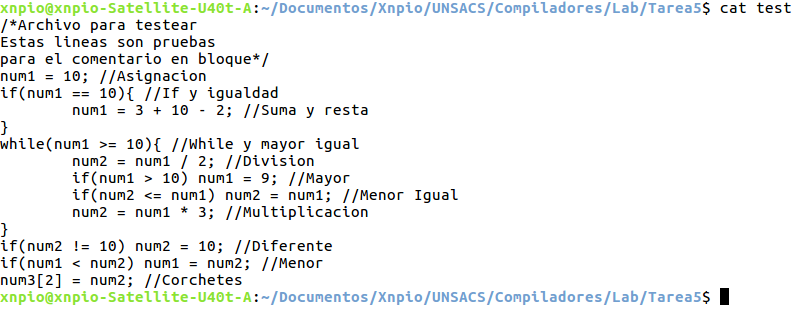
\includegraphics[scale = 0.5]{1.png}
 \caption{Archivo del experimento}
\end{figure}
\begin{figure}[H]
 \centering
 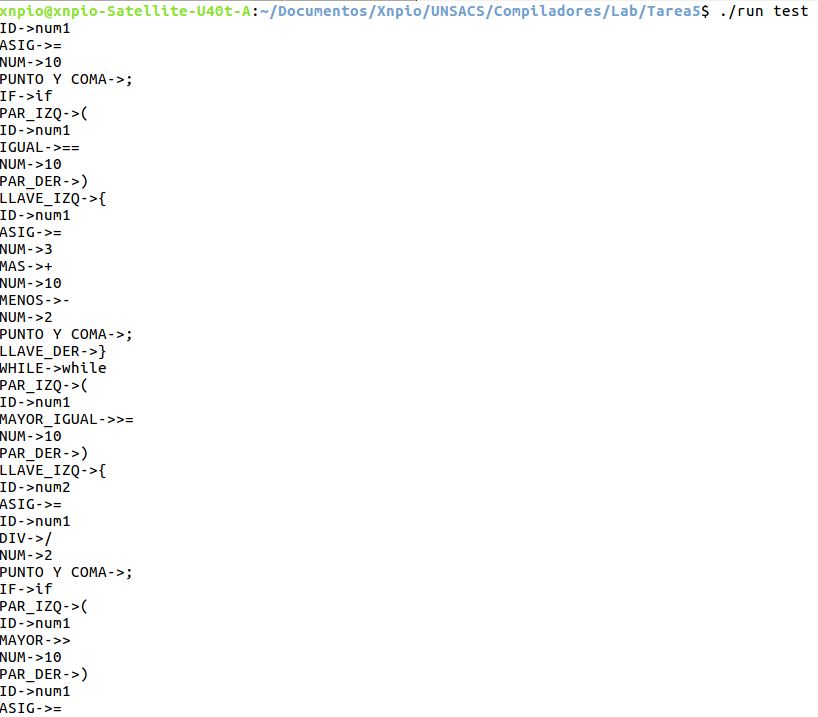
\includegraphics[scale = 0.5]{2.png}
\end{figure}
\begin{figure}[H]
 \centering
 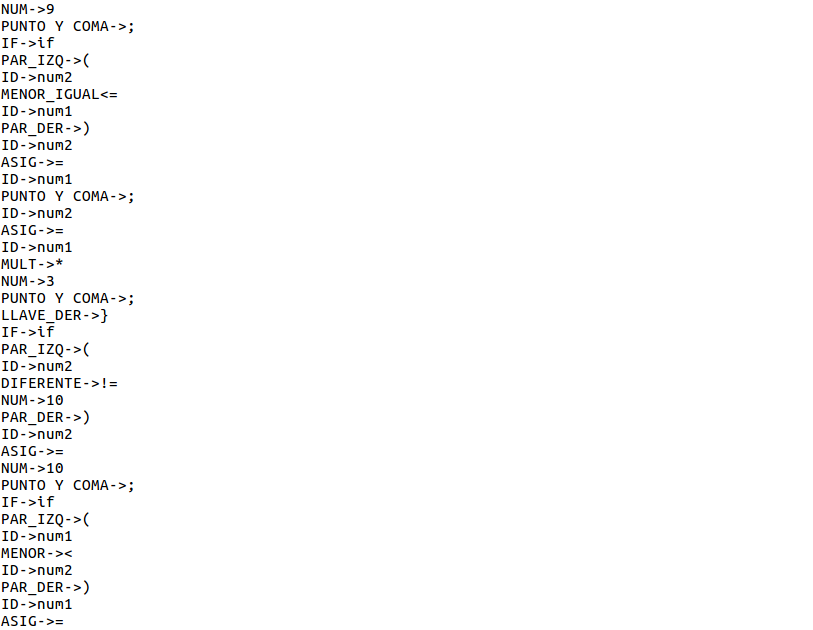
\includegraphics[scale = 0.5]{3.png}
\end{figure}
\begin{figure}[H]
 \centering
 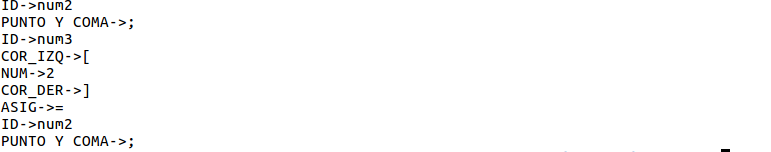
\includegraphics[scale = 0.5]{4.png}
 \caption{Resultado del programa}
\end{figure}





\end{document}

